\section{Examples}
\subsection{Pseudocode}
Give a Turing machine that decides $L = \left\{ww ~|~ w\in \left\{0, 1\right\}^\ast\right\}$
\begin{minted}{python}
On input x:
  if |x| is odd: REJECT
  let n = |x| / 2
  for i in 0, 1, ..., n - 1:
    if x[i] != x[n + i]: REJECT
  ACCEPT
\end{minted}
\subsection{Dovetailing}
Give a Turing machine that recognizes

\hspace{5mm}$L = \left\{\langle M \rangle ~|~ M \textrm{ is a Turing machine and } L(M) \neq \varnothing\right\}$

Is it decidable? The following fails
\begin{minted}{python}
On input <M>:
  for w in Sigma*:
    simulate M on w # may loop before accepting
    if M accepts: ACCEPT
\end{minted}
To recognize it we need dovetailing
\begin{minted}{python}
On input <M>:
  W = set of strings lexicographically sorted
  for i in range(len(W)):
    for j in range(i):
      (Run M on W[i] for _ in range(i - j))
      if M accepts: ACCEPT
\end{minted}
$\forall i, j$ we will eventually run at least enough $j$ steps for $M$
to halt and accept.
\subsection{Show Language is Context Free}
\subsubsection{Example 1}
Consider binary operation $\nabla$ where $A$ and $B$ are each regular
languages

$A\nabla B = \left\{xy ~|~ x \in A, y \in B, \textrm{ and } |x| = |y|\right\}$

$A \circ B = \left\{ xy ~|~ x \in A, y \in B\right\}$ is regular

Concatenation in an NFA joins $M_A$ and $M_B$ inline with $\epsilon$
transitions. To construct PDA enter $M_A$ by pushing a start symbol to
stack. Inside $M_A$ push a tracking symbol to stack. Inside $M_B$ pop
tracking symbols out of stack. Finally, exit $M_B$ accepting symbols by
popping starting symbol. Formally:

$M_A = \left(Q_A, \Sigma, \delta_A, q_0^A, F_A\right)$,
$M_B = \left(Q_B, \Sigma, \delta_B, q_0^B, F_B\right)$

$PDA: M = \left(Q, \Sigma, q_0, \delta, \left\{q_f\right\}, \left\{\ast, \$\right\}\right)$

$Q = Q_A \cup Q_B \cup \left\{q_0, q_f\right\}$

$\delta(q_0, \epsilon, \epsilon) = \left\{\left(q_0^A, \$\right)\right\}$

$\delta(q_A, \sigma, \epsilon) = \left\{\left(\delta_A(q_A, \sigma), \ast\right)\right\}$

$\delta(f_A, \epsilon, \epsilon) = \left\{\left(q_0^B, \epsilon\right)\right\}$

$\delta(q_B, \sigma, \ast) = \left\{\left(\delta_B(q_B, \sigma), \epsilon\right)\right\}$

$\delta(f_B, \epsilon, \$) = \left\{\left(q_f, \epsilon\right)\right\}$

where $q_A \in Q_A,~ q_B \in Q_B,~ f_A \in F_A,~ F_B \in F_B$ and
$\sigma\in\Sigma$
\vspace{1mm}
\subsubsection{Example 2}
Prove that the intersection of a context-free language and a regular
language is context-free.

Given CFL $L$ and a regular language $R$, let PDA $P$ accept $L$ and NFA
$N$ accept $R$. Define

$P = (Q_1, \Sigma, \delta_1, \Gamma, F_1)$

$N = (Q_2, \Sigma, \delta_2, F_2)$

We can construct a PDA $P^N$ that represents the cross-product
construction of $P$ and $N$ such that:

$Q = Q_1 \times Q_2$

$(f_1, f_2) \in F$ s.t. $f_1 \in F_1$ and $f_2 \in F_2$

$\delta\left(\left(q_{1},q_{2}\right),x,y\right) \in $

\hspace{10mm}$\left\{\left(q_{1}',q_{2}'\right)\textrm{ s.t. }q_{1}'\in\delta_{1}\left(q_{1},x,y\right)\textrm{ and }q_{2}'\in\delta_{2}\left(q_{2},x\right)\right\}$

Because we can construct a PDA that accepts $P^N$, then $L\cap R$ is
context-free.
\subsubsection{Example 3}
Let $\Sigma$ and $\Gamma$ be finite alphabets. A \textbf{substitution}
is a mapping
$\sigma: \Sigma \to \mathcal{P}(\Gamma^*)$

where every symbol $a \in \Sigma$ is assigned a language $\sigma(a)
\subseteq \Gamma^*$.

For a word $w = a_1 a_2 \dots a_k \in \Sigma^*$ define

\hspace{1cm}$\sigma(w) = \sigma(a_1) \sigma(a_2) \dots \sigma(a_k)$,

i.e. the concat of langs $\sigma(a_i)$. For a lang $L\subseteq\Sigma^*$
set

\hspace{1cm}$\sigma(L) = \bigcup_{w\in L}\sigma(w)$

Prove that if $L$ is context-free and every lang $\sigma(a)$, $a
\in\Sigma$, is context-free, then $\sigma(L)$ is context-free.

For this problem, we forgot to add that the substitution should have
been defined also to map the empty string to the empty string. In any
case, because $L$ is context-free, there exists a grammar $G$ for $L$.
For every symbol-language mapping, because each of these languages is
context-free, we can also define grammars for those languages as well.
Thus, we can construct a new grammar such that for every terminal symbol
for $G$, we can replace it with the grammar associated with the language
mapping for that symbol.

\subsection{Show Language is Decidable}
\subsubsection{Example 1}
Show that Turing decidable langs are closed under concatenation. Let
$L_1$ and $L_2$ be decidable.

Let $L_1$ and $L_2$ be Turing-decidable languages and let $M_1$ and
$M_2$ be TMs that decide those languages respectively. We will construct
a TM $M_3$ that decides a concatenation as follows:

1. For input string $w$, consider all two substring partitions:
$\left\{(x,y) ~|~ w = xy: x,y \in \Sigma^\ast\right\}$

2. For each two substring partitions, simulate $M_1$ on $x$ and $M_2$ on
$y$ for all two substring partitions. If both $M_1$ and $M_2$ accept $x$
and $y$, then $M_3$ accepts. Otherwise, if this doesn't occur for all
two substring partitions, then $M_3$ rejects.

Because there are a finite number of two substring partitions, the
computation for \#1 will halt. Additionally, because both $M_1$ and
$M_2$ are decidable, they will halt for any string, and \#2 will halt.
Thus, $M_3$ will halt.

As a result, for our proof of correctness, we merely have to show for $w
\in L_1\circ L_2 \implies w \in L(M_3)$ and $w\notin L_1\circ L_2
\implies w \notin L(M_3)$

The "proof" is just a verbose description of the above.
\subsubsection{Example 2}
Let $L = \left\{\langle A, R \rangle ~|~ A \textrm{ is a DFA}, R
\textrm{ is a regex}, L(A) = L(R) \right\}$. Then $L$, is a language
containing all strings that are encoded by a DFA $A$ and a regular
expression $R$. Show that $L$ is decidable.

This is essentially a $EQ_{\textrm{DFA}}$ problem. To show this formally.

There exists a TM $M_1$ that decides this language because
$EQ_{\textrm{DFA}}$ is decidable. We will construct a TM $M_2$ as follows:

1. Processes input $\langle A, R \rangle$ and check for valid
concatenation of DFA and regular expression encoding. Otherwise, reject.

2. Convert $\langle R \rangle$ to an equivalent NFA and then DFA. Then encode this DFA as $\langle B \rangle$ and concatenate it with $\langle A \rangle$ so that we have $\langle A, B \rangle$.

3. Simulate $M_1$ on $\langle A, B \rangle$. If $M_1$ accepts, then $M_2$ will accept. If $M_1$ rejects then $M_2$ will reject.

Steps 1 and 2 are finite operations and will halt. Step 3 will halt as
well because $M_1$ is decidable and will halt on any input. Thus $M_2$
will halt.

Our proof of correctness, needs to show that for $w \in L \implies w \in
L(M_2)$ and $w \notin L \implies w \notin L(M_2)$.

If $w \in L$, then $w$ is a valid encoding $\langle A, R \rangle$. Thus, steps 1 and 2 will proceed without issue. Additionally, $\langle A, B \rangle$ would be in $EQ_{\textrm{DFA}}$because $L(B) = R$ and thus accepted by $M_1$. Thus, steps 1-2 will proceed without issue but $M_2$ wil reject $w$ in step 3.

As a result, because there exists a TM that accepts the language and halts on every input, the language is decidable.

\subsection{Show Language is Recognizable}
\subsubsection{Example 1}
Show that the Turing-recognizable languages are closed under
intersection. Remember closed means that if you have Turing-recognizable
language, $L_1$, and Turing-recognizable language, $L_2$, show that
their intersection is Turing-recognizable.

Let $L_1$ and $L_2$ be Turing-recognizable languages and let $M_1$ and
$M_2$ be TMs that recognize those languages respectively. We will
construct a TM $M_3$ that recognizes the intersection as follows: $M_3$
on input $w$:

\hspace{1mm}(a) Simulates $M_1$ on $w$. If $M_1$ rejects, $M_3$ rejects.
If M1 accepts, then go to b.

\hspace{1mm}(b) Simulate $M_2$ on $w$. If $M_2$ accepts, then accept.
Otherwise, reject.

Note that $M_3$ may reject string by looping forever in step a or b and
that would be acceptable to recognize the intersection.

For our proof correctness, we have to show for $w \in L_1 \cap L_2
\implies w \in L(M_3)$ and $w \notin L_1 \cap L_2 \implies w \notin
L(M_3)$

If $w \in L_1 \cap L_2$, then both $M_1$ and $M_2$ accept $w$. Thus,
$M_3$ will accept $w$.

If $w \notin L_1 \cap L_2$, then $M_1$ or $M_2$ does not accept $w$ (or
both). It may be explicitly rejected or loop forever by either $M_1$ or
$M_2$. Either way, $M_3$ will not accept $w$.

This, because there exists a Tm that accepts the intersection, the
intersection is Turing-recognizable.

\subsection{Show Language is Undecidable}
\subsubsection{Example 1}
Let $L = \left\{\langle M \rangle ~|~ L(M) \textrm{ is
context-free}\right\}$. Prove that $L$ is undecidable.

We want a reduction from $\textrm{HALT} \leq_m L$. In other words
$f(\langle M, x \rangle) = \langle T \rangle$. If $f$ exists it implies
that

$\langle M, x \rangle\in\textrm{HALT} \iff \langle T \rangle \in L$.


\begin{minted}{python}
def T(w): # w is some input
  # this is just so that L(T) is not empty if M loops
  if w == 0^n 1^n 0^n: ACCEPT
  simulate M(x)
  ACCEPT # L(T) = Sigma*
\end{minted}

Thus if $M$ would halt, then $L(T) = \Sigma^\ast$, and if $M$ loops
$L(T) = {0^n1^n0^n ~|~ n\geq 0}$ which are CFL and non-CFL respectively.
Since $f$ is computable then this is a valid reduction and $L$ is
undecidable.

\subsection{Decidable or Undecidable?}
\subsubsection{Example 1}
Let $L = \left\{\langle M \rangle ~|~ \exists k. \forall s\in L(M),
\left|s\right|\leq k\right\}$. In other words, the set of all Turing
machines that only accept bounded-length strings. Is $L$ decidable or
undecidable.

\begin{minted}{python}
def T(w): # w is some input
  (simulate M(x) for _ in range(len(w)))
  # accepts when L(T) = Sigma*
  if M accepted or rejected: REJECT
  # accepts when L(T) = {w in Sigma* | len(w) < n}
  if M had not finished: ACCEPT
\end{minted}

Since $M(x)$ halts if and only if $\langle T \rangle \in L$, then
$\textrm{HALT} \leq_m L$ and $L$ is undecidable.
\subsubsection{Example 2}
Let $L_k = \left\{\langle M \rangle ~|~ M\textrm{'s tape head index }\leq k\right\}$. Is $L_k$ decidable or
undecidable.

That is a property of a TM and not of a language so let's try to build a
TM that accepts it to show $L_k$ is decidable.

\begin{minted}{python}
def N(<M>): # w is some input
  for w in {bounded strings of length <= k}
    simulate M(w)
    during simulation:
      if M head >= k: REJECT
      elif M halts: continue
      else:
        track the state of M
        if we encounter a cycle: continue
  ACCEPT # all w have been tried
\end{minted}

This TM is possible; therefore, $L_k$ is decidable.

\subsubsection{Example 3}
Consider $B = \left\{\langle M \rangle ~|~ L(M) \textrm{ is
finite}\right\}$. Is $B$ decidable or undecidable?

Not that the set of all finite languages is a langauge property. From
Rice's Theorem, this implies that $B$ is undecidable.

\subsubsection{Example 4}
Consider $C = \left\{\langle M \rangle ~|~ M \textrm{ halts within 500
steps}\right\}$. Is $C$ decidable or undecidable?

This is decidable. We just need a computer program to run the $M$ for at
most 500 steps to determine whether $\langle M \rangle$ is in the
langauge.
\subsubsection{Example 5}
Let $F = \left\{\langle M, N \rangle ~|~ M \textrm{ accepts on estring
that } N \textrm{ does not}\right\}$. Prove that $F$ is undecidable. Do
not use Rice's Theorem.

We will reduce $A_{\textrm{TM}}$ to $F$. We will transform the input $\langle M, w \rangle$ by creating the following two functions:
\begin{minted}{text}
For input x:
  if x == w:  evaluate M on w
  else: REJECT
\end{minted}
\begin{minted}{text}
For input x:
  REJECT
\end{minted}
The encodings for these two functions $\langle A, B \rangle$ will be
concatenated and provided to $F$. Note that $L(B) = \varnothing$.

If $\langle M, w \rangle \in A_{\textrm{TM}}$, then $L(A) = w$ and
$\langle A, B \rangle\in F$. If $\langle M,w \rangle\notin
A_{\textrm{TM}}$, then $L(A) = \varnothing$ and $\langle A, B
\rangle\notin F$.

Because we have reduced $A_{\textrm{TM}}$ to $F$ and $A_{\textrm{TM}}$
is undecidable, this implies that $F$ is undecidable.

\subsection{Reductions}
\subsubsection{Example 1}
Consider the function $EMPTY : \left\{0, 1\right\}^\ast$ that takes a
DFA as input and outputs 1 if the language of the DFA is empty. That is,
$EMPTY(D) = 1$ if $D$ describes a DFA ( under some encoding the
representation is not important) that does not accept any string. Define
$EQUIVALENT: EQUIVALENT(D, D') = 1$ if $D(x) = D'(x), \forall x$. Give a
reduction from $EQUIVALENT$ to $EMPTY$.

This problem looks at language from the perspective of functions, which
is another way of looking at languages. Whenever a function evaluates
the input string to 1, then the input string is part of the language,
and whenever a function evaluates the input string to 0, then the input
string is not part of the language. Thus, to reduce $EQUIVALENT$ to
$EMPTY$, we have to show that $w \in L(EQUIVALENT) \iff f(w) \in
L(EMPTY)$.

Valid inputs to $EQUIVALENT$ are two DFA encodings. Given valid inputs,
we shall transform them in the following way: generate the DFA encoding,
which iss equivalent to the intersection of the first DFA and the
complement of the second. As previously discussed in class, we can
generate this new DFA in a computable manner. If an invalid input is
provided, then we will just generate some fixed non-emtpy DFA.

Consider $w \in L(EQUIVALENT)$. This implies that $f(w)$ will be the DFA
encoding associated with an empty DFA. Thus $f(w) \in L(EMPTY)$.

Consider $w\notin L(EQUIVALENT)$. This implies that $f(w)$ be the DFA
encoding associated ith a non-empty DFA. This $f(w) \in L(EMPTY)$.

\subsection{Rice's Theorem Quick Guide}
Given $M$
\begin{center}
  \resizebox{8cm}{!}{
  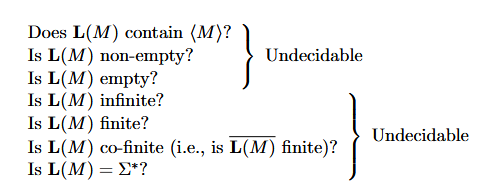
\includegraphics[]{images/rice-01.png}
  }
\end{center}

Properties of TMs
\begin{center}
  \resizebox{8cm}{!}{
  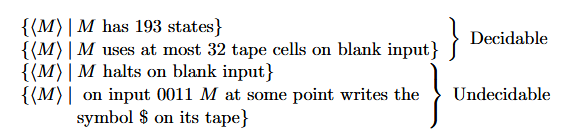
\includegraphics[]{images/rice-02.png}
  }
\end{center}